%2multibyte Version: 5.50.0.2953 CodePage: 1252

\documentclass[bigger,handout]{beamer}
%%%%%%%%%%%%%%%%%%%%%%%%%%%%%%%%%%%%%%%%%%%%%%%%%%%%%%%%%%%%%%%%%%%%%%%%%%%%%%%%%%%%%%%%%%%%%%%%%%%%%%%%%%%%%%%%%%%%%%%%%%%%%%%%%%%%%%%%%%%%%%%%%%%%%%%%%%%%%%%%%%%%%%%%%%%%%%%%%%%%%%%%%%%%%%%%%%%%%%%%%%%%%%%%%%%%%%%%%%%%%%%%%%%%%%%%%%%%%%%%%%%%%%%%%%%%
\usepackage{amssymb}
\usepackage{amsfonts}
\usepackage{amsmath}
\usepackage{mathpazo}
\usepackage{hyperref}
\usepackage{multimedia}
\usepackage{graphicx}

\setcounter{MaxMatrixCols}{10}
%TCIDATA{OutputFilter=LATEX.DLL}
%TCIDATA{Version=5.50.0.2953}
%TCIDATA{Codepage=1252}
%TCIDATA{<META NAME="SaveForMode" CONTENT="1">}
%TCIDATA{BibliographyScheme=Manual}
%TCIDATA{Created=Monday, October 27, 2008 15:56:24}
%TCIDATA{LastRevised=Monday, May 01, 2017 12:51:58}
%TCIDATA{<META NAME="GraphicsSave" CONTENT="32">}
%TCIDATA{<META NAME="DocumentShell" CONTENT="Other Documents\SW\Slides - Beamer">}
%TCIDATA{Language=American English}
%TCIDATA{CSTFile=beamer.cst}

\newenvironment{stepenumerate}{\begin{enumerate}[<+->]}{\end{enumerate}}
\newenvironment{stepitemize}{\begin{itemize}[<+->]}{\end{itemize} }
\newenvironment{stepenumeratewithalert}{\begin{enumerate}[<+-| alert@+>]}{\end{enumerate}}
\newenvironment{stepitemizewithalert}{\begin{itemize}[<+-| alert@+>]}{\end{itemize} }
\usetheme{Madrid}
\usecolortheme{beaver}
\usefonttheme{professionalfonts}
\input{tcilatex}
\setbeamertemplate{navigation symbols}{}
\begin{document}

\title[47-809: Control]{Optimal Control approach to dynamic models}
\subtitle{Judd Sections 10.6-10.7}
\author[David Childers]{David Childers (thanks to Y. Kryukov, K. Judd, and U. Doraszelski)}
\institute[CMU]{CMU, Tepper School of Business}
\date[Apr 17]{Apr 17, 2023}
\maketitle

\section{Functional equations}

 
 
\begin{frame}%
 
\frametitle{The Plan}

\begin{itemize}
\item Dynamic Programming approach:

\begin{itemize}
\item Rewrite the model as Bellman equation

\item Solve for policy and value functions
\end{itemize}

\item \textbf{Optimal control approach}:

\begin{itemize}
\item Hamiltonian and Pontryagin optimality conditions

\item Derive ODE for state and control (policy), \newline
as functions of time

\item Then derive ODE for policy function
\end{itemize}

\item Today:

\begin{itemize}
\item Finite horizon; Example: lifetime savings

\item Infinite horizon; Example: optimal growth

\item Examples are cont. time, cont. state, determ. transition

\item Bonus: Stochastic case: "Forward Backward SDE"
\end{itemize}
\end{itemize}

 
 
\end{frame}%
 
 
 
\begin{frame}%
 
\frametitle{Optimal Control problem with finite horizon}

\begin{equation*}
\begin{array}{rc}
\max_{u} & \int_{0}^{T}e^{-\rho t}\pi (x,u,t)dt+g(x(T)) \\ 
\text{subject to:} & \dot{x}=f(x,u,t),\quad x(0)=x_{0},%
\end{array}%
\end{equation*}%
where

\begin{stepitemize}
\item $t$ is time, $\rho >0$ is the discount rate

\item $x\in \mathbb{R}^{n}$ is a vector of state variables;

\item $u\in \mathbb{R}^{m}$ is a vector of control variables;

\item $\pi :\mathbb{R}^{n+m+1}\rightarrow \mathbb{R}$ is the payoff flow;

\item $g:\mathbb{R}^{n}\rightarrow \mathbb{R}$ is the terminal payoff; and

\item $f:\mathbb{R}^{n+m+1}\rightarrow \mathbb{R}^{n}$ is the law of motion 
\newline
(state transition process).
\end{stepitemize}

 
 
\end{frame}%
 
 
 
\begin{frame}%
 
\frametitle{Solution: Pontryagin conditions}

Hamiltonian = "Lagrangian for functions":%
\begin{equation*}
H(x,u,\lambda ,t)=\pi (x,u,t)+\lambda ^{\top }f(x,u,t),
\end{equation*}%
where $\lambda \in R^{n}$ is a vector of costate variables
(\textquotedblleft multipliers\textquotedblright )

\begin{enumerate}
\item The optimality condition: $u=\arg\max H(x,u,\lambda ,t)$ 
\begin{equation*}
\text{FOC: }0=\tfrac{\partial H}{\partial u}=\pi _{u}(x,u,t)+\lambda ^{\top
}f_{u}(x,u,t).
\end{equation*}

\item Law of motion: $\dot{x}=\frac{\partial H}{\partial \lambda }%
\Rightarrow \dot{x}=f(x,u,t)$.

\item Costate equation: $\dot{\lambda}=\rho \lambda -\frac{\partial H}{%
\partial x}=$\newline
$=\rho \lambda -\pi _{x}(x,u,t)-\lambda ^{\prime }f_{x}(x,u,t)$

\item Initial condition: $x(0)=x_{0}.$

\item Transversality condition (TVC): $\lambda (T)=g^{\prime }(x(T));$

\begin{enumerate}
\item In BVP: $g(x(T))\equiv 0$; impose $x(T)=x_{T}$ instead \newline
$\Rightarrow $ terminal condition on $x(T)$ replaces the TVC.
\end{enumerate}
\end{enumerate}

 
 
\end{frame}%
 
 
 
\begin{frame}%
 
\frametitle{Example: Life-cycle consumption}

Let $A(t)$ be assets that consumer holds at time $t$:%
\begin{equation*}
\begin{array}{rc}
\max_{c} & \int_{0}^{T}e^{-\rho t}u(c)dt \\ 
\text{subject to} & \dot{A}=f(A)+w-c, \\ 
& A(0)=A(T)=0%
\end{array}%
\end{equation*}

\begin{enumerate}
\item Hamiltonian: $H=u(c)+\lambda \left[ f(A)+w-c\right] $

\item The optimality condition $H_{c}=u^{\prime }(c)-\lambda =0$

\begin{enumerate}
\item Differentiate w.r.t. time: $\dot{\lambda}=u^{\prime \prime }(c)\dot{c}$%
.
\end{enumerate}

\item Costate: $\dot{\lambda}=\rho \lambda -H_{A}=\rho \lambda -\lambda
f^{\prime }\left( A\right) $
\end{enumerate}

Use 2 \& 2.a to eliminate $\lambda $ from 3

 
 
\end{frame}%
 
 
 
\begin{frame}%
 
\frametitle{Example continued}

\begin{stepitemize}
\item Combine optimality and costate eq-ns: 
\begin{equation}
\dot{c}=\frac{u^{\prime }(c)}{u^{\prime \prime }(c)}\left( \rho -f^{\prime
}(A)\right) ,  \label{eq:Cdot}
\end{equation}

\item Law of motion and boundary conditions%
\begin{eqnarray}
\dot{A} &=&f(A)+w-c,\quad  \label{eq:Adot} \\
A(0) &=&A(T)=0  \label{eq:Abound}
\end{eqnarray}

\item (\ref{eq:Cdot})-(\ref{eq:Abound}) form a BVP

\item Shooting: pick $c_{0}$ to ensure $A(T)=0$
\end{stepitemize}

 
 
\end{frame}%
 
 
 
\begin{frame}%
 
\frametitle{Phase diagram (Figure 10.2)}

\begin{itemize}
\item Axes are current level of consumption and capital

\item Short arrows represent signs of $\dot{c}=c^{\prime }\left( t\right) $
and $\dot{A}$

\item $c=f\left( A\right) $ line is really $c=f\left( A\right) +w$; (\ref%
{eq:Adot}) tells us that:

\begin{itemize}
\item $\dot{A}=0$ on the line

\item $\dot{A}>0$ (arrows right) below the line, as $f(A)+w>c$

\item $\dot{A}<0$ (arrows left) above the line, as $f(A)+w<c$
\end{itemize}

\item Assume $f^{\prime }(A)>\rho $. Then (\ref{eq:Cdot}) implies $\dot{c}>0 
$,\newline
so there are only up arrows, and no down ones.

\item Curved arrows = \emph{trajectories} $\left\{ A\left( t\right) ,c\left(
t\right) \right\} _{t\in \left[ 0,T\right] }$ for different $c_{0}$

\begin{itemize}
\item Their direction is governed by short arrows

\item Tip of the arrow corresponds to $A\left( T\right) ,c\left( T\right) $,

\item We reach $A\left( T\right) =0$ by adjusting $c_{0}$ ($c_{L}$, $c_{H}$,
etc.)
\end{itemize}
\end{itemize}

 
 
\end{frame}%
 
\begin{frame}%
\frametitle{Fig 10.2: Phase diagram in life cycle model}

\scalebox{0.45}{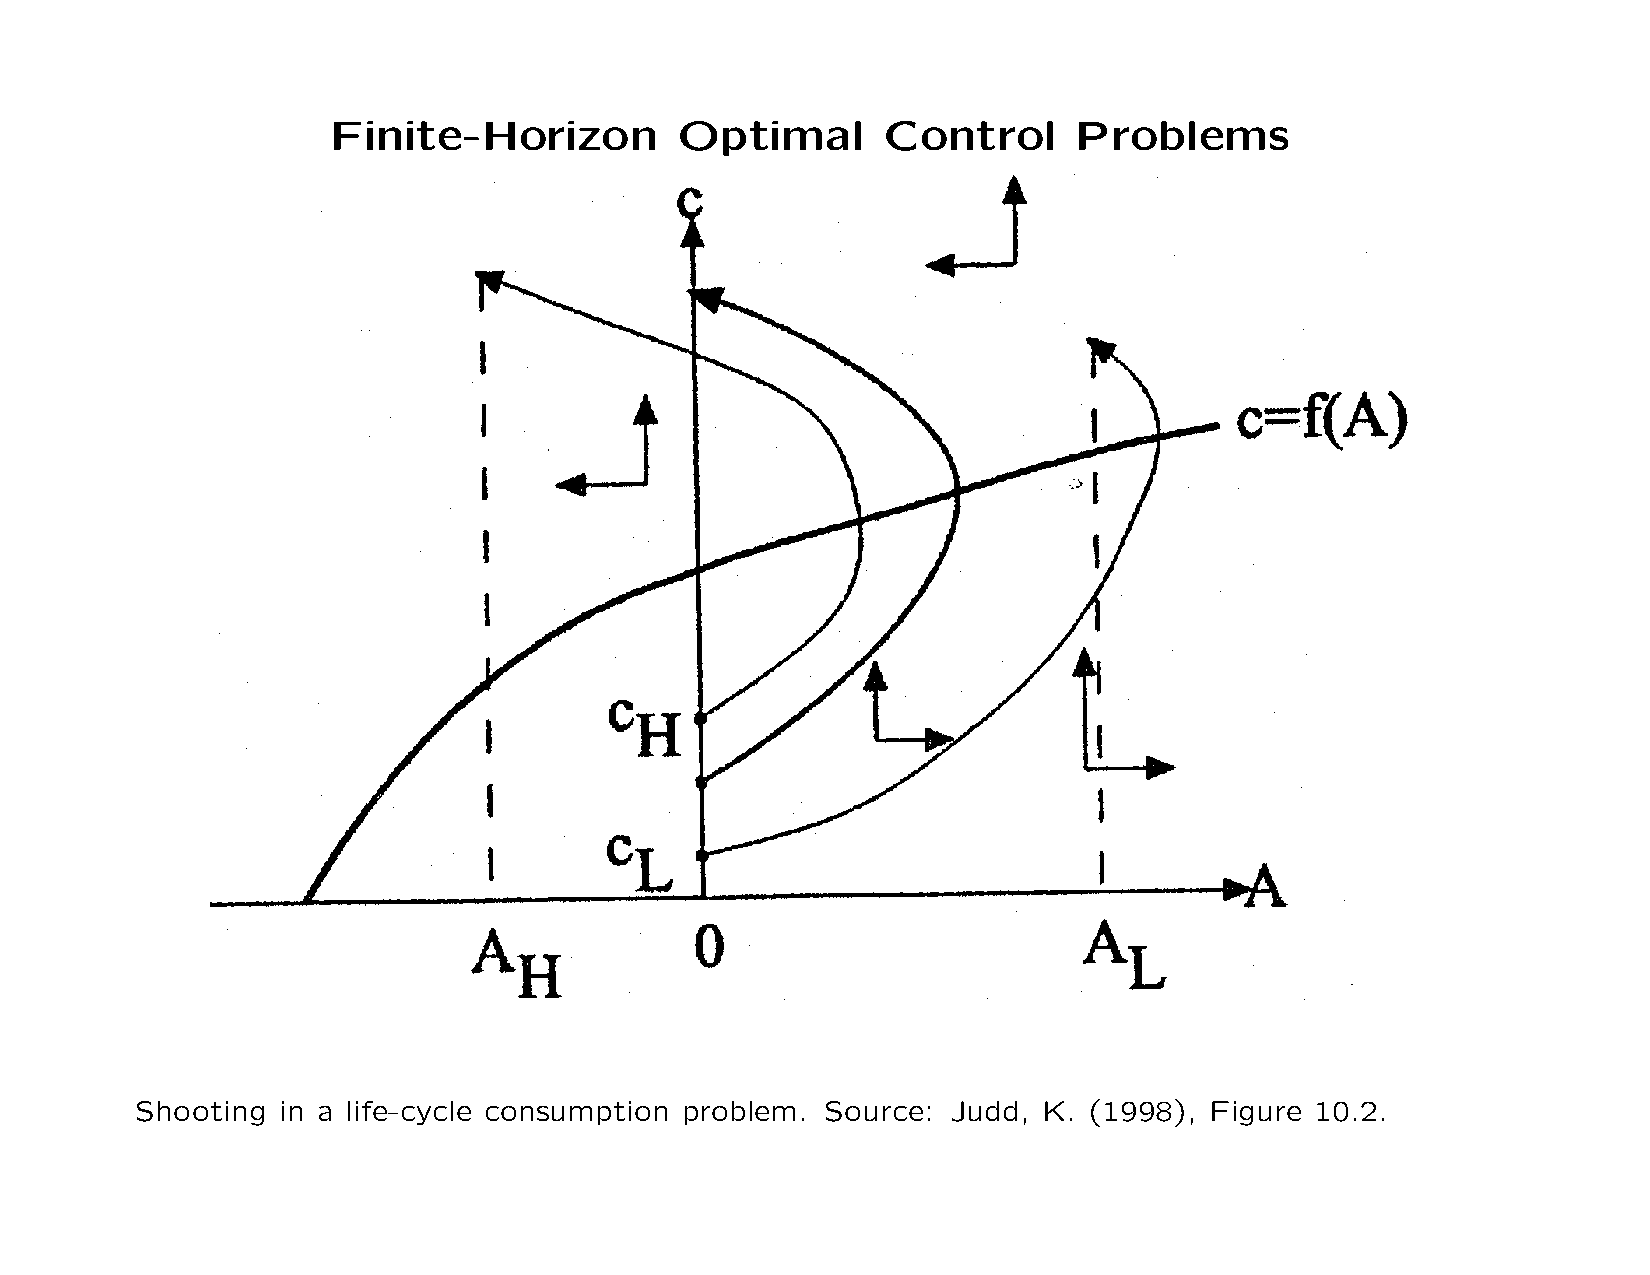
\includegraphics{shootingmethod.pdf}}
 
\end{frame}%
 
 
\begin{frame}%
 
\frametitle{Aside on modeling choices}

\begin{itemize}
\item Finite horizon should be justified

\begin{itemize}
\item Truncating an infinite-horizon problem creates terminal effects
\end{itemize}

\item In most cases, "death" is random

\begin{itemize}
\item Adjustment to discount factor: $\tilde{\beta}=\beta \Pr \{survival\}$

\item Poisson arival of death in cont. time
\end{itemize}

\item Attempt at justifying Lifecyle problem:

\begin{itemize}
\item $T=$ retirement age: require $A\left( T\right) =\bar{A}>0$ 
\end{itemize}

\item Infinite-horizon models should have steady state

\begin{itemize}
\item Or stable (limiting) distribution of states

\item It should be inside the modeled interval

\item Otherwise, value function is driven by value at the edge of the
interval, which is undetermined

\item If known to \emph{asymptote} to steady state, can pretend it arrives at large finite $T$: justify by a turnpike theorem   

\item Solution to infinite growth: rescale state (e.g. K per
capita)
\end{itemize}
\end{itemize}

 
 
\end{frame}%
 
 
 
\begin{frame}%
 
\frametitle{Optimal control with Infinite horizon }

No more terminal period $T$ 
\begin{equation*}
\begin{array}{rl}
\max_{u} & \int_{0}^{\mathbf{\infty }}e^{-\rho t}\pi (x,u,t)dt \\ 
\text{subject to:} & \dot{x}=f(x,u,t),\quad x(0)=x_{0},%
\end{array}%
\end{equation*}

The system of ODEs consists of:

\begin{stepitemize}
\item Optimality condition: $\frac{\partial H}{\partial u}=0$

\item Law of motion: $\dot{x}=\frac{\partial H}{\partial \lambda }%
=f(x,U(x,\lambda ,t),t)$.

\item Initial condition: $x(0)=x_{0}.$

\item Costate equation: $\dot{\lambda}=\rho \lambda -\frac{\partial H}{%
\partial x}$

\item \textbf{TVC}: $\lim_{t\rightarrow \infty }e^{-\rho t}|\lambda
(t)^{T }x(t)|<\infty $

\begin{itemize}
\item Satisfied if variables converge to a \textbf{steady state}: \newline
$\left( u^{\ast },x^{\ast }\right) :\dot{u}=\dot{x}=0$
\end{itemize}
\end{stepitemize}

 
 
\end{frame}%
 
 
 
\begin{frame}%
 
\frametitle{Example: Optimal growth}

\begin{stepitemize}
\item Recall the optimal growth problem%
\begin{equation*}
\begin{array}{rl}
\max_{c} & \int_{0}^{\infty }e^{-\rho t}u(c)dt \\ 
\text{subject to:} & \dot{k}=f(k)-c,\qquad k(0)=k_{0}%
\end{array}%
\end{equation*}

\item The optimality condition $0=u^{\prime }(c)-\lambda $ implies $\dot{%
\lambda}=u^{\prime \prime }(c)\dot{c}$.

\item Thus, the system of ODEs is 
\begin{gather*}
\dot{c}=\frac{u^{\prime }(c)}{u^{\prime \prime }(c)}\left( \rho -f^{\prime
}(k)\right) \\
\dot{k}=f(k)-c \\
k(0)=k_{0} \\
\lim_{t\rightarrow \infty }e^{-\rho t}|\lambda (t)k(t)|<\infty
\end{gather*}

\item TVC is satisfied if $\forall \epsilon>0$ $\exists T \text{ s.t. } \forall t\geq T$, $\left|\dot{k}(t)\right|,\left|\dot{c}(t)\right|<\epsilon$
\end{stepitemize}

 
 
\end{frame}%
 
 
 
\begin{frame}%
 
\frametitle{Steady state \& Phase diagram}

\begin{stepitemize}
\item The steady state $(k^{\ast },c^{\ast })$ satisfies $\dot{k}=\dot{c}=0$

\item Implies%
\begin{eqnarray*}
f(k^{\ast })-c^{\ast } &=&0 \\
\rho -f^{\prime }(k^{\ast }) &=&0
\end{eqnarray*}

\item Algorithm 10.3: Shoot for $c(T)=c^{\ast }$, where $T$ is the first
time such that $\dot{k}(T)\leq 0$ or $\dot{c}(T)\leq 0$.

\item Phase diagram (Figure 10.3, assume $k_{0}<k^{\ast }$):

\begin{itemize}
\item If $c_{0}$ is too large, then the path crosses the $\dot{k}=0$ line, 
\newline
so that $k(t)$ keeps falling and $c(t)$ keeps rising.

\item If $c_{0}$ is too small, the path crosses the $\dot{c}=0$ line, 
\newline
so that $k(t)$ keeps rising and $c(t)$ keeps falling.
\end{itemize}
\end{stepitemize}

 
 
\end{frame}%
 
 
 
\begin{frame}%
 
\frametitle{Reverse shooting}

\begin{stepitemize}
\item Problem: $k(T)$ too sensitive to $c(0)$ when $T$ is large.

\item Solution -- reverse shooting (from $T$ to $0$): \newline
Initial state is not very sensitive to terminal state

\item Reverse the direction of time ($s=-t$), conditions change sign: 
\begin{gather*}
\dot{c}=-\frac{u^{\prime }(c)}{u^{\prime \prime }(c)}\left( \rho -f^{\prime
}(k)\right) , \\
\dot{k}=-\left( f(k)-c\right) ,
\end{gather*}

\item $\Rightarrow $ Phase diagram in figure 10.4

\item The unstable manifold of the new system \newline
is the stable manifold of the old system.

\item So shooting succeeds
\end{stepitemize}

 
 
\end{frame}%

\begin{frame}%
 
\frametitle{Shooting and Reverse Shooting}

\scalebox{1.0}{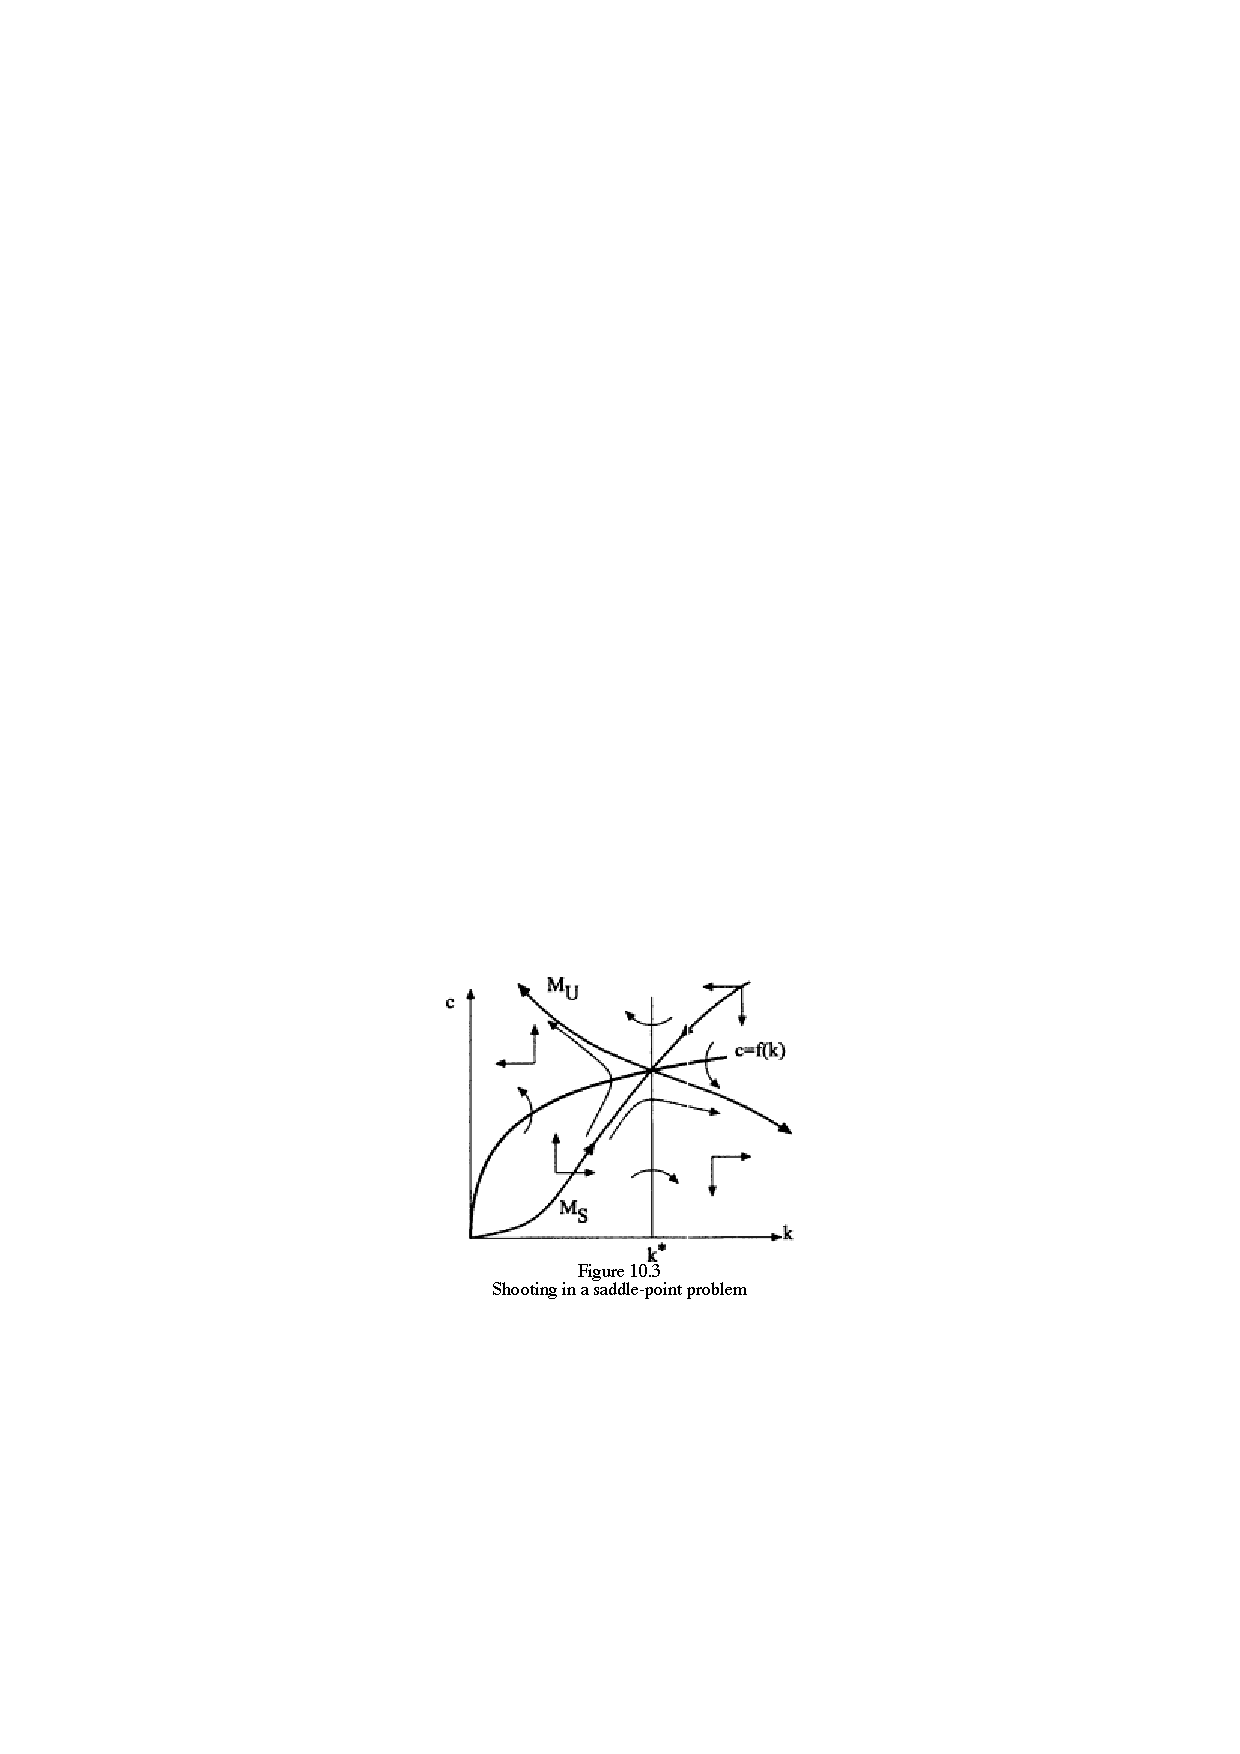
\includegraphics{saddleshooting.pdf} 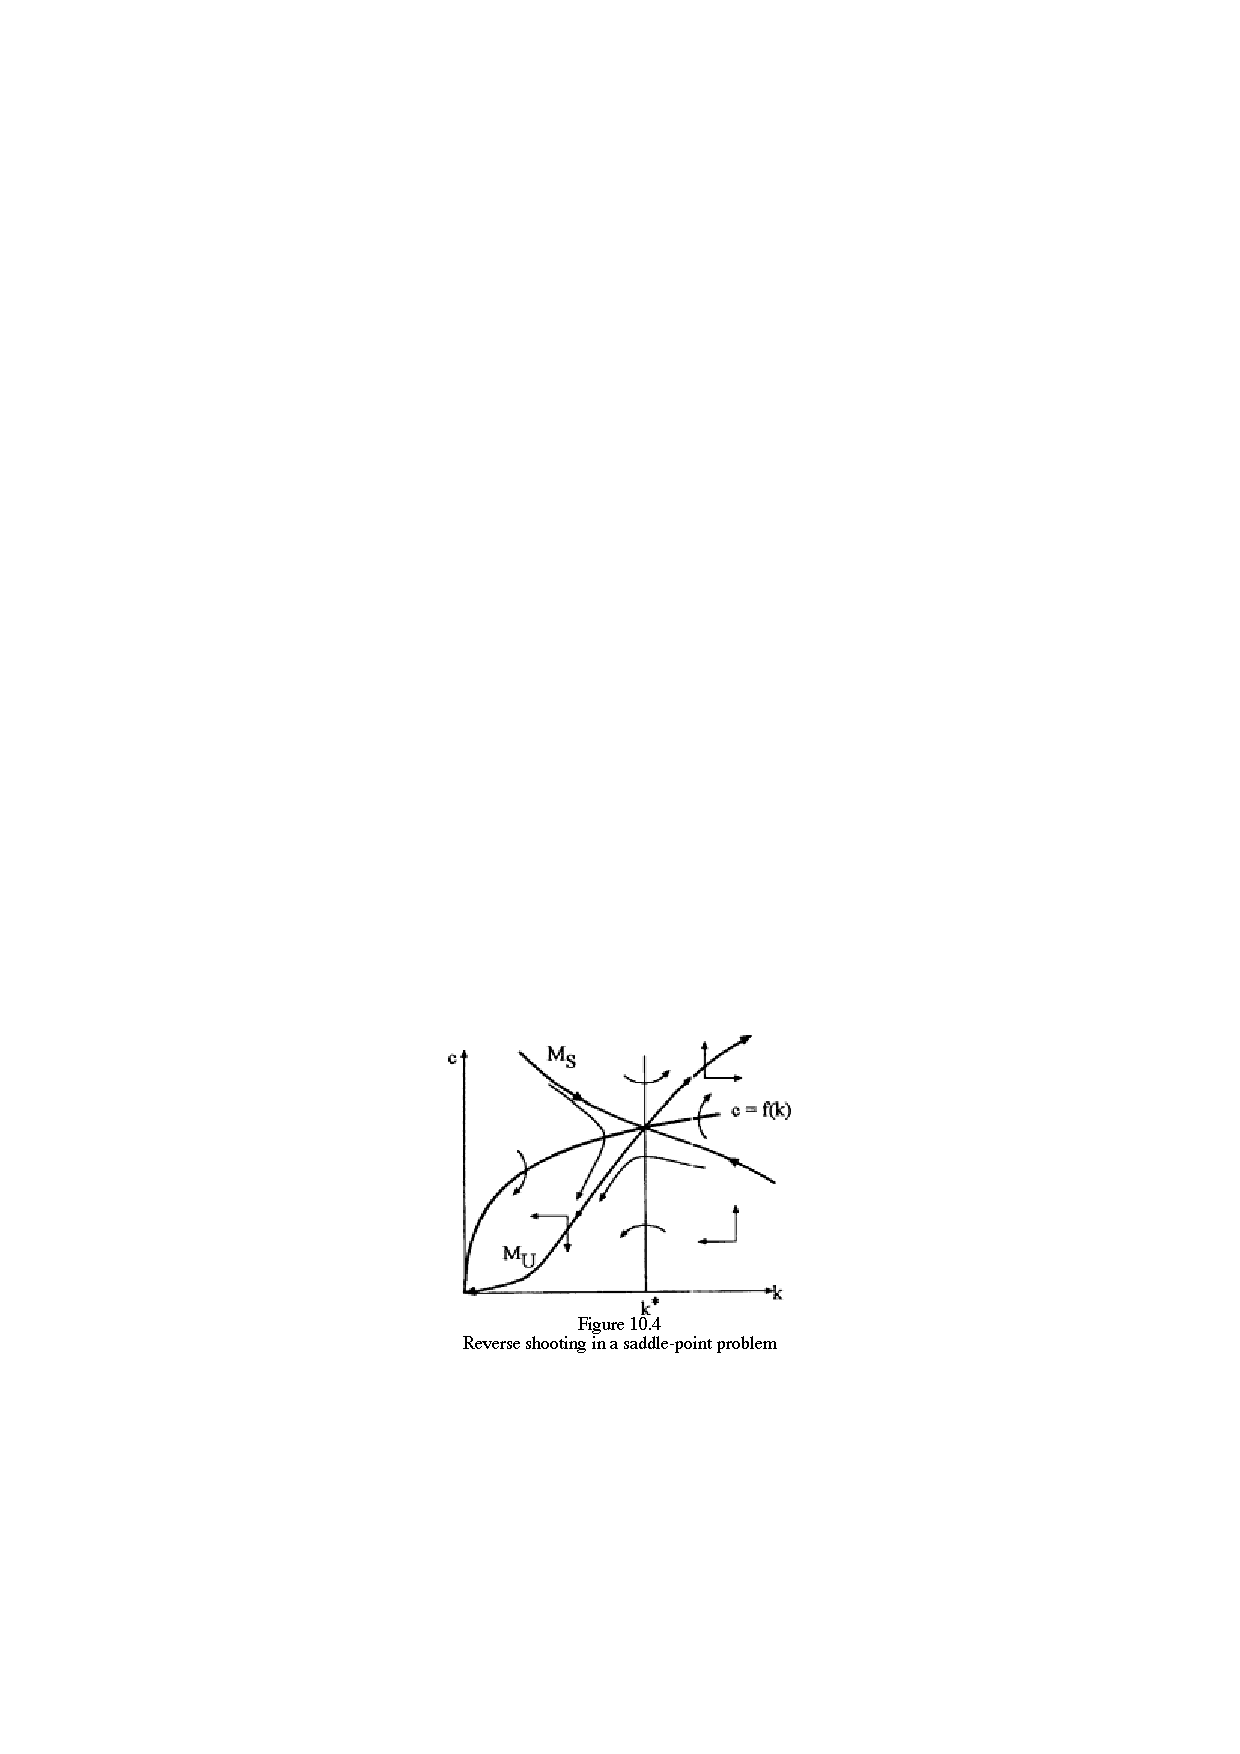
\includegraphics{reverseshooting.pdf}} 
 
\end{frame}%
 
 
 
% \begin{frame}%
%  
% \frametitle{Policy function}
% 
% \begin{itemize}
% \item There is no $t$ in conditions; only $\partial t$
% 
% \item We can define the policy function $C(k)$ such that $c(t)=C(k(t))$.
% 
% \item Defined by ODE: 
% \begin{equation}
% C^{\prime }(k)=\frac{\dot{c}}{\dot{k}}=\frac{u^{\prime }\left( C\left(
% k\right) \right) }{u^{\prime \prime }\left( C\left( k\right) \right) }\frac{%
% \rho -f^{\prime }\left( k\right) }{f(k)-C\left( k\right) }  \tag{*}
% \end{equation}
% 
% \begin{itemize}
% \item Initial condition: $C\left( k^{\ast }\right) =c^{\ast }$
% \end{itemize}
% 
% \item Only problem: $C^{\prime }\left( k^{\ast }\right) =?$
% \end{itemize}
% 
%  
%  
% \end{frame}%
%  
%  
%  
% \begin{frame}%
%  
% \frametitle{Solving policy function ODE}
% 
% \begin{itemize}
% \item l'Hopital's rule. If $h\left( \bar{z}\right) =g\left( \bar{z}\right)
% =0 $, then%
% \begin{equation*}
% \lim_{\bar{z}}\frac{h\left( z\right) }{g\left( z\right) }=\frac{h^{\prime
% }\left( \bar{z}\right) }{g^{\prime }\left( \bar{z}\right) }
% \end{equation*}
% 
% \item Apply to $\left[ \rho -f^{\prime }\left( k\right) \right] /\left[
% f(k)-C\left( k\right) \right] $ in (*):%
% \begin{equation*}
% C^{\prime }(k^{\ast })=\frac{u^{\prime }\left( c^{\ast }\right) }{u^{\prime
% \prime }\left( c^{\ast }\right) }\frac{-f^{\prime \prime }\left( k^{\ast
% }\right) }{f^{\prime }(k^{\ast })-C^{\prime }\left( k^{\ast }\right) }
% \end{equation*}
% 
% \item This leads to quadratic eq-n, with two solutions
% 
% \begin{itemize}
% \item Which one to use?
% \end{itemize}
% 
% \item One you have $C^{\prime }(k^{\ast })$, use finite difference method
% twice: \newline
% for $k\leq k^{\ast }$ and for $k\geq k^{\ast }$.
% \end{itemize}
% 
%  
%  
% \end{frame}%
%  
%  
%  
% \begin{frame}%
%  
% \frametitle{Policy function via projection}
% 
% \begin{itemize}
% \item Approximate $C\left( k\right) $ as $\hat{C}\left( k;a\right) $
% 
% \item Residual function -- directly from (*):%
% \begin{equation*}
% \tilde{R}\left( k;a\right) =\frac{u^{\prime }\left( \hat{C}\left( k;a\right)
% \right) }{u^{\prime \prime }\left( \hat{C}\left( k;a\right) \right) }\frac{%
% \rho -f^{\prime }\left( k\right) }{f(k)-\hat{C}\left( k;a\right) }-\hat{C}%
% ^{\prime }\left( k;a\right)
% \end{equation*}
% 
% \item Or transform to avoid $1/\hat{C}\left( k;a\right) $:%
% \begin{equation*}
% R\left( k;a\right) =\frac{u^{\prime }\left( \hat{C}\left( k;a\right) \right) 
% }{u^{\prime \prime }\left( \hat{C}\left( k;a\right) \right) }\left( \rho
% -f^{\prime }\left( k\right) \right) -\hat{C}^{\prime }\left( k;a\right) %
% \left[ f(k)-\hat{C}\left( k;a\right) \right]
% \end{equation*}
% 
% \item Use any projection approach: collocation, least squares
% 
% \item Can add $\hat{C}\left( k^{\ast };a\right) =c^{\ast }$ as a collocation
% condition, \newline
% or use it to find the constant term ($a_{0}$)
% \end{itemize}
% 
%  
%  
% \end{frame}%

\begin{frame}%

\frametitle{Stochastic Case: Forward Backward SDE}

\begin{equation*}
\begin{array}{rc}
\max_{u} & \int_{0}^{T}\pi (x,u,t)dt+g(x(T)) \\
\text{subject to:} & dx=f(x,u,t)dt+\sigma(x,u,t)dW,\quad x(0)=x_{0},%
\end{array}%
\end{equation*}%


\begin{itemize}
\item Generalized Hamiltonian
\end{itemize}
\begin{equation*}
H(x,u,\lambda,z,t) = \pi(x,u,t)+\lambda^{T}f(x,u,t)+Tr(\sigma^{T}(x,u,t)z)
\end{equation*}
\begin{enumerate}
\item Optimality: $\hat{u}_t=\arg\max H(x_t,u,\lambda,z_t,t)$

\item Law of motion: $dx_t=f(x_t,\hat{u}_t,t)dt+\sigma(x_t,\hat{u}_t,t)dW_t$.
 
\item Costate equation: $d\lambda_{t}=-\nabla_{x}H(x_t,\hat{u}_t,\lambda_t,z_t,t)dt+z_{t}dW_t$
\item Initial condition: $x(0)=x_{0}$
\item Transversality condition (TVC): $\lambda (T)=g^{\prime }(x(T))$

\end{enumerate}

\begin{itemize}
\item Solve SDE system for $(x_t,u_t,\lambda_t,z_t)$: 1 extra costate
\item where $\lambda_t=\nabla_{x}V(x_t,t)$, $z_t=\sigma(x_t,\hat{u}_t,t)^{T}\text{Hess}_{x}V(x_t,t)$
\end{itemize}



\end{frame}

% \begin{frame}
% 
% \frametitle{Stochastic Pontryagin Principle}
% 
% 
% 
% \end{frame}
 
 
\begin{frame}%
 
\frametitle{Opt. control vs. Dyn.programming}

\textbf{The Good}:

\begin{itemize}
\item No need to solve for value function, or depend on covergence

\item Provides timepaths ($c\left( t\right) ,k\left( t\right) $) directly

\item Works well with finite-horizon models
\end{itemize}

\textbf{The Bad}:

\begin{itemize}
\item Stochastic transition case difficult: "Forward Backward SDE"

\begin{itemize}
\item Additional costate $z_t$ is stochastic 

\item It has to be specified as function of transition process
\end{itemize}
\end{itemize}

\textbf{The Ugly:}

\begin{itemize}
\item Derivation-intensive, can be numerically unstable
\end{itemize}

 
 
\end{frame}

\begin{frame}%
 
\frametitle{References}

\begin{itemize}

\item Judd Ch. 10

\item Morton Kamien and Nancy Schwartz (2012) \emph{Dynamic optimization: the calculus of variations and optimal control in economics and management}
\begin{itemize}
\item Classic with proofs and derivations
\end{itemize}

\item Hu and Lauri\`{e}re \href{https://arxiv.org/abs/2303.10257}{"Recent Developments in Machine Learning Methods for Stochastic Control and Games"}
\begin{itemize}
\item Survey with numerical methods including for FBSDE approach
\end{itemize}

\end{itemize}

\end{frame}


 

\end{document}
